\documentclass[../main.tex]{subfiles}

\begin{document}
    \begin{center}
        \subsection{Рассчет минимальной энергии Оже-процесса}
    \end{center}

    Одним из способов увеличения интенсивности стимулированного излучения является повышение разности насселенностей,
    что в случае подобных структур приводит к задаче увеличения времени жизни носителей заряда,
    для как можно большей эффективности процесса излучательной рекомбинации. 
    Всвязи с этим важно иметь возможность оценить минимальную энергию, носителей, при которой возможен Оже-процесс.

    Как известно, Оже-рекомбинация является трехчастичным процессом. Причем в таком процессе могут участвовать квазичастицы разных 
    подзон - в таком случае выражение для частоты переходов будет содержать матричный элемент перехода, который оказывается не 
    равным нулю. Кроме того выражение для этой частоты будет содержать в дельта функцию импульсов, что соответствует закону сохранения:
    \begin{equation}
        W \propto \delta(\vec{k}_{1i} + \vec{k}_{2i} + \vec{k}_{1j} - \vec{k}_{3i});
    \end{equation}

    При этом индексы $i,j$ - нумеруют типы квазичастиц (дырки или электроны). Все квазичастицы могут находиться в разных подзонах, иначе говоря
    в данном случае не существует какого-то дополнительного закона сохранения, связанного с отбором некоторых веток дисперсионного соотношени.
    $\vec{k}_{1i},~\vec{k}_{2i},~\vec{k}_{1j}$ - импульсы начальных частиц, $\vec{k}_{3i}$
    - конечной.


    

    Здесь $i,j$ - типы квазичастиц (дырки и электроны), $\vec{k}_{1i},~\vec{k}_{2i},~\vec{k}_{1j}$ - импульсы начальных частиц, $\vec{k}_{3i}$
    - конечной.

        Здесь $i,j$ - два сорта квазичастиц (в частности, возможно ). Необходимо отметить наличие связи частот перехода:
        \begin{equation}
            \omega(\vec{k}_i^{(1)},~\vec{k}_i^{(2)},~\vec{k}_j \rightarrow \vec{k}_i^{'(2)})
                \propto \delta_3 (\vec{k}_i^{(1)} + \vec{k}_i^{(2)} + \vec{k}_j - \vec{k}_i^{'(2)}) \cdot 
                \delta \left(\varepsilon_i(\vec{k}_i^{(1)}) + \varepsilon_i (\vec{k}_i^{(2)}) + \varepsilon_j (\vec{k}_j)
                    - \varepsilon_i (\vec{k}_i^{'(2)})\right);
        \end{equation}
            
        Очевидно, что в общем виде эта задача сложна по нескольким причинам:
        \begin{itemize}
            \item амплитуда такого рассеяния может быть найдена как с
                помощью диаграмной техники Келдыша \cite{AugerDiagrams}, 
                так и с помощью метода последовательных приближений \cite{SucApprAnd, SucApprAgr},
                однако в обоих случаях имеется сильное расхождение
                теории и эксперимента [ссылка];
            \item подобные рассчеты весьма вычислительно сложны и не могут
                быть использованы в поиске оптимального дизайна структуры.
        \end{itemize}

        Однако есть и куда более простой способ - отыскание порога Оже-процесса.
        С учетом наличия возможности рассчета дисперсионного соотношения методом Кейна 8x8
        \cite{HgCdTeCalcZholudev} и наличия законов сохранения в таких
        процессах задача может быть сведена к оптимизации некой характеристической
        функции.

        Рассмотрим некоторые общие свойства процессаб в котором участвуют две
        квазичастицы типа $i$ и одна типа $j$. В таком случае выберем три подзоны для 
        $i$ частиц (двух начальных и конечной), которым соответствуют импульсы 
        $\vec{k}_1,~\vec{k}_2,~\vec{k}_f$ и дисперсионные 
        соотношения $\varepsilon_1,~\varepsilon_2,~\varepsilon_f$ и одну для частицы типа $j$,
        соответствующую $\vec{k}_j,~\varepsilon_j$ (подразумевается, что 
        $\varepsilon_j \geq 0, \forall \vec{k}_j$). Будем оптимизировать (минимизировать) функцию, 
        характеризующую "кинетическую" энергию частицы, оставшейся после участия в акте Оже-рекомбинации 
        (что эквивалентно оптимизации "кинетической" энергии трех частиц до взаимодействия):
        
        \begin{equation}
            \varkappa = \varepsilon_f(\vec{k}_1 + \vec{k}_2 + \vec{k}_j) - E_g.
        \end{equation}

        С учетом условий:
        %\bea
        %    \vec{k}_1 + \vec{k}_2 + \vec{k}_j - \vec{k}_f = 0;\\
        %    \varepsilon_1(\vec{k}_1) + \varepsilon_2(\vec{k}_2) + \varepsilon_j(\vec{k}_j) - \varepsilon_f(\vec{k}_f) = 0;
        %\eea

        Подставим закон сохранения импулься сразу и воспользуемся методом неопределённых множителей:
        \begin{equation}
            L = \varepsilon_f(\vec{k}_1 + \vec{k}_2 + \vec{k}_j) - E_g + \lambda \cdot \left(\varepsilon_1(\vec{k}_1) + 
            \varepsilon_2(\vec{k}_2) + \varepsilon_j(\vec{k}_j) - \varepsilon_f(\vec{k}_1 + \vec{k}_2 + \vec{k}_j)\right);
        \end{equation}

        Тогда, дифференциируя, получим важный  вывод: для минимальной энергии необходимо соблюдение условия
        \begin{equation}
            \nabla \varepsilon_1(\vec{k}_1) = \nabla \varepsilon_2(\vec{k}_2) = \nabla \varepsilon_h(\vec{k}_h);
        \end{equation}
        Это можно интерперетировать, как необходимость равенства групповых скоростей квазичастиц.
        
        В случае рассмотрения
                прямозонной ситуации и небольших импульсов имеем 
                    $\varepsilon (\vec k) = \frac{\hbar^2}{2} \vec k \widehat{m^{-1}} \vec k + \varepsilon_0$.
                Тогда в силу симметричности тензора обратных масс получим $\nabla \varepsilon = \hbar^2 \widehat{m^{-1}} \vec k$.

        Теперь рассмотрим ситуацию изотропного дисперсионного соотношения $\varepsilon(\abs{\vec k})$,
        очевидно в таком случае для минимизации энергии требуется коллинеарность всех импульсов. 
        В таком случае можно достаточно просто численно определить пороговую энергию Оже процесса, что и было сделано.

        Для этого входные данные считываются и по ним строится интерполяция,
        в виде сплайна третьего порядка. В дальнейшем производится оптимизация функции с условием:
        \begin{eqnarray}
            \varkappa  = \varepsilon_f(k_1 + k_2 + k_h) - E_g;\\
            \varepsilon_1(k_1) + \varepsilon_2(k_2) + \varepsilon_h(k_h) - \varepsilon_f(k_1 + k_2 + k_h);
        \end{eqnarray}

        Также стоит отметить, что зачастую удобно использовать сплайны Акимы \cite{AkimaSplines}, поскольку они позволяют существенно уменьшить
        численные артефакты, связанные с переколебаниями сплайна. Это позволяет значит увеличить точность вычислейний, а также убрать ложные
        участки дисперсионного соотношения, имеющие необходимую радиальную компоненту градиента.

        Следует отметит, что ввиду наличия большого количества локальных минимумов функции процесс её оптимизации представляется далеко нетривиальной задачей.
        В ходе работы были опробованы различные методы глобальной оптимизации - основанные на стохастических процессах (метод роя частиц, метод 
        симуляции холодного отжига), а также методы сокращения исследуемой области. Однако наиболее эффективным является метод разбиения 
        дисперсионного соотношения на участки, имеющие одинаковый знак первой производной и выбор наборов таких участков,
        на которых может бьыть реализована ситуация совпадения групповых скоростей квазичастиц. В дальнейшем выбиралась произвольная точка этого диапазона
        и от нее проводилась оптимизация методом AUGLAG \cite{AuglagOptim} с наложенными ограничниями при помощи пакета NLOpt \cite{NLopt}.

        В результате такого рассмотрения были получены интересные закономерности в случае гетероструктур, содержащих ямы с большой концентрацией кадмия.
        В частности было выявлено несколько характерных паттернов.
        
        \begin{figure}[h!]
            \begin{minipage}[h]{0.3\linewidth}
                \begin{center}
                    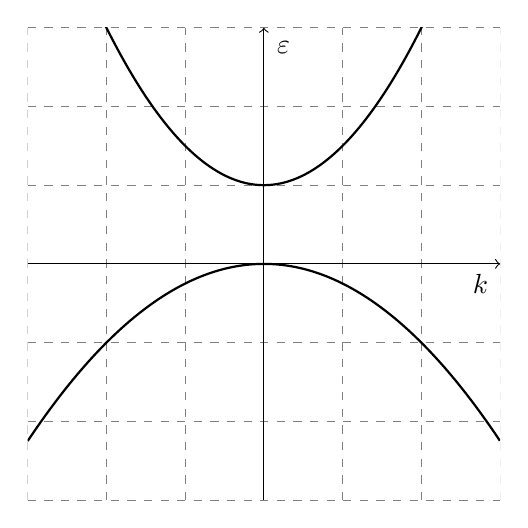
\begin{tikzpicture}
                        \clip (-3, -3) rectangle (3, 3);
                        \draw [help lines, dashed, thin] (-3, -3) grid (3, 3);
                        \draw [->, thin] (-3, 0) -- (3, 0);
                        \draw (2.75, -0.25) node {$k$};
                        \draw [->, thin] (0, -3) -- (0, 3);
                        \draw (0.25, 2.75) node {$\varepsilon$};
                        \draw [domain = -3:3, samples = 200, thick] plot ({\x}, {\x * \x * 0.5 + 1.});
                        \draw [domain = -3:3, samples = 200, thick] plot ({\x}, {-\x * \x * 0.25});
                    \end{tikzpicture}
                \end{center}
            \end{minipage}
            \hfill
            \begin{minipage}[h]{0.3\linewidth}
                \begin{center}
                    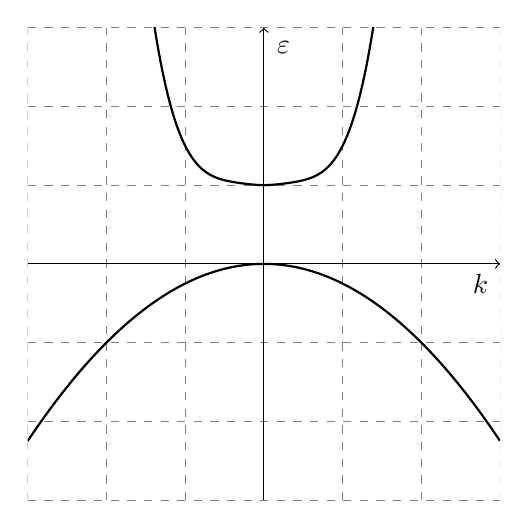
\begin{tikzpicture}
                        \clip (-3, -3) rectangle (3, 3);
                        \draw [help lines, dashed, thin] (-3, -3) grid (3, 3);
                        \draw [->, thin] (-3, 0) -- (3, 0);
                        \draw (2.75, -0.25) node {$k$};
                        \draw [->, thin] (0, -3) -- (0, 3);
                        \draw (0.25, 2.75) node {$\varepsilon$};
                        \draw [domain = -3:3, samples = 200, thick] plot ({\x}, {0.5 * pow(\x, 2) - abs(pow(\x, 3)) + pow(\x, 4) + 1.});
                        \draw [domain = -3:3, samples = 200, thick] plot ({\x}, {-\x * \x * 0.25});
                    \end{tikzpicture}
                \end{center}
            \end{minipage}
            \hfill
            \begin{minipage}[h]{0.3\linewidth}
                \begin{center}
                    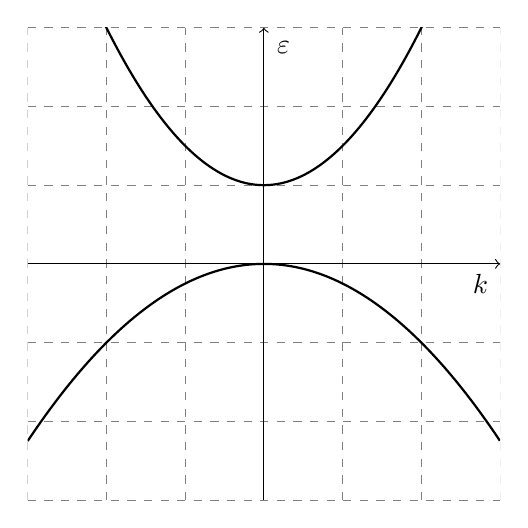
\begin{tikzpicture}
                        \clip (-3, -3) rectangle (3, 3);
                        \draw [help lines, dashed, thin] (-3, -3) grid (3, 3);
                        \draw [->, thin] (-3, 0) -- (3, 0);
                        \draw (2.75, -0.25) node {$k$};
                        \draw [->, thin] (0, -3) -- (0, 3);
                        \draw (0.25, 2.75) node {$\varepsilon$};
                        \draw [domain = -3:3, samples = 200, thick] plot ({\x}, {\x * \x * 0.5 + 1.});
                        \draw [domain = -3:3, samples = 200, thick] plot ({\x}, {-\x * \x * 0.25});
                    \end{tikzpicture}
                \end{center}
            \end{minipage}
        \end{figure}

        Можно видеть, что наличие дополнительных максимумов в дисперсионных соотношениях для электронов
        может значительно снижать порог Оже-процессов, за счет участия в рекомбинации квазичастиц с разными фазовыми,
        но одинаковыми групповыми скоростями. Это может приводить к существенно более быстрой зависимости
        интенсивности фотолюминисцентного изулучения от температуры.

        Причем в структурах с большим содержанием кадмия в квантовых ямах наблюдается тенденция к образованию
        подобных побочных максимумов. 
    \newpage
\end{document}